\documentclass{article}
\usepackage[utf8]{inputenc}
\usepackage[margin=0.8in]{geometry}
\usepackage{amsmath}
\usepackage{graphicx}
\usepackage{amsthm}
\usepackage{algorithm}
\usepackage{algpseudocode}
\usepackage{enumitem}
\usepackage{verbatim}
\usepackage{tikz-qtree}
\usepackage{color, soul}
\usepackage{makecell}
% \usepackage{qtree}
\graphicspath{ {./} }

\title{CS190I HW2 Report}
\author{Matthew Ho}
\date{January 2022}

\usepackage{listings}
\usepackage{color}

\definecolor{codegreen}{rgb}{0,0.6,0}
\definecolor{codegray}{rgb}{0.5,0.5,0.5}
\definecolor{codepurple}{rgb}{0.58,0,0.82}
\definecolor{backcolour}{rgb}{0.95,0.95,0.92}

\lstdefinestyle{style1}{
}

\algnewcommand{\var}{\texttt}

\lstset{
    commentstyle=\color{codegreen},
    keywordstyle=\color{magenta},
    numberstyle=\tiny\color{codegray},
    stringstyle=\color{codepurple},
    basicstyle=\ttfamily\footnotesize,
    breakatwhitespace=false,         
    breaklines=true,                 
    captionpos=b,                    
    keepspaces=true,                 
    numbers=left,                    
    numbersep=2pt,                  
    showspaces=false,                
    showstringspaces=false,
    showtabs=false,                  
	xleftmargin=5.0ex,
    tabsize=2,
	breaklines=true,
    postbreak=\mbox{\textcolor{red}{$\hookrightarrow$}\space}
}


\begin{document}
\maketitle

\section{Collaboration}
Did you receive any help whatsover from anyone in solving this assignment? \textbf{No}\\
Did you give any help whatsoever to anyone in solving this assignment? \textbf{No}

\section{Report}
\begin{center}
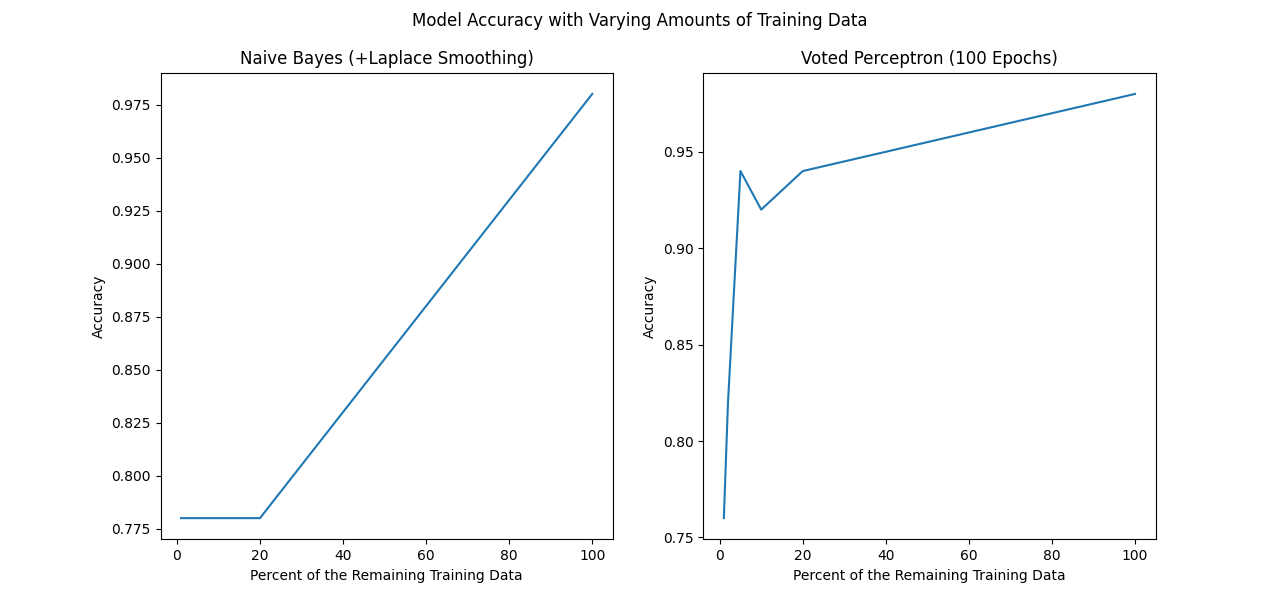
\includegraphics[scale=0.5]{report_graphs}
\end{center}
First of all it should be noted that the last 10 percent of training data is unbalanced (11/50 are fake), so classifiers benefit from being skewed towards guessing non-fake. The Naive Bayes classifier had the same performance for each percentage except for 100. This may be because the maximum likelihood estimates used in the posterior probability computation are more reliable with larger sample sizes.

On the other hand, the Voted Perceptron's performance increased greatly from the 5 initial training examples (1 percent of the remaining data). This makes sense as the model gets significantly more opportunities to adjust its weights from the initial 0 values. The dip from 0.94 to 0.92 accuracy from 5 to 10 percent of remaining training data marks one fewer correct prediction on the n=50 ``test" set, so I attribute the dip to chance.


\end{document}
